\section{Umsetzung}
\subsection{Technologie und Plattform}
In der Problembeschreibung zu dieser Arbeit wurden die Anforderungen an eine SmartHome Lösung diskutiert. In der anschliessenden Marktanalyse wurde openHAB als Grundlage zur Umsetzung unseres Projekts evaluiert. OpenHAB erfüllt die geforderten Kritierien, wie Herstellerunabhängigkeit, Installierbarkeit und Flexibilität. Cloudseitig wird MS Azure Cloud zur Persistierung von Events verwendet.

\subsection{Einführung openHAB}
Das System openHAB wird eingesetzt, um verschiedene Home-Automatisierungssysteme unter einen Hut zu bringen. Um dies zu erreichen müssen Lösungen für die vier Disziplinen Konnektivität, User Interface, Automatisierung und Persistenz gefunden werden. In den nächsten Abschnitten werden diese Disziplinen kurz beschrieben.

\subsubsection{Konnektivität}
Mit Konnektivität ist gemeint, wie die Sensoren/Aktoren integriert werden können. Es braucht ein Konzept um Protokolle miteinander kompatibel zu machen. Nehmen wir als Beispiel den Use Case \emph{L03: Event Kontaktsensor}. An einem Fenster wird ein Kontaktsensor angebracht, der bei jedem Öffnen oder Schliessen den Status bekannt gibt. OpenHAB muss einerseits das verwendete Protokoll verstehen und zudem die Daten in eine interne, abstrakte Form übersetzen, sodass Herstellerspezifische Details vor dem restlichen System verborgen bleiben. Ein weiters Beispiel ist Use Case \emph{L05: Aktor: Lampe}. Hierbei müssen keine Events gelesen, sondern Commands geschickt werden, da es sich bei der Lampe um einen Aktor handelt. Dazu muss openHAB auch den umgekehrten Fall beherrschen, nämlich aus einer internen Repräsentation des Commands in diejenige des Protokolls der Lampe zu übersetzen und letztlich auch die Lampe erreichen können. Durch Konnektivität ist es also möglich, SmartHome Zubehör von verschiedenen Herstellen in openHAB einzubinden. 

\subsubsection{User Interface}
Nehmen wir an, der Fensterkontakt und die Lampe aus dem vorherigen Abschnitt sind von zwei völlig verschiedenen Herstellern. Der Status des Fensterkontakts soll bei der Verwendung ohne openHAB über eine Website im Browser ausgelesen werden können. Das Steuern der Lampe geschehe mittels einer eigens dafür vorgesehenen App. Dank dem Konzept zur Konnektivität können aber beide Geräte auch über openHAB zugegriffen werden. Einen echten Vorteil hat man dadurch aber nur, wenn es auch ein User Interface dazu gibt. Denn dann hat man alle Geräte in einer Smartphone- oder Web App vereint. OpenHAB benötigt demnach eine Möglichkeit um User Interfaces für verschiedene Clients zu gestalten.

\subsubsection{Automatisierung}
Durch die Konnektivität und das User Interface kann also SmartHome Zubehör von verschiedenen Herstellern in einer einzigen Anwendung verwendet werden. Das alleine ist schon ein grosser Mehrwert. Doch es fehlt noch etwas der smarte Teil des SmartHomes. Interessant wird es nämlich dann, wenn die verschiedenen Geräte sich gegenseitig beeinflussen sollen. Nehmen wir den Bewegungsmelder aus Use Case L04 hinzu. Sobald er eine Bewegung registriert soll die Lampe eingeschaltet werden. Es sind aber auch wesentlich komplexere Szenarien denkbar. Damit solche automatisierten Vorgänge stattfinden können benötigt openHAB eine Rule Engine. Die Grundlage dazu bildet die interne Repräsentation der Sensoren und Aktoren, die bereits durch die Konzepte zur Konnektivität geschaffen wurde.

\subsubsection{Persistenz}
Wenn Events gelesen und Commands gesendet werden, dann handelt es sich dabei um Momentaufnahmen. Im User Interface könnte man beobachten, wenn der Status des Fensterkontakts von offen auf zu wechselt. Doch was ist, wenn man wissen möchte, wann das Fenster zuletzt geöffnet wurde? Aus diesem Grund reicht es nicht, Events lediglich zu verarbeiten, sondern sie müssen auch persistiert werden. Zudem können manche Sensoren wie der Fensterkontakt möglicherweise nur immer einen Statuswechsel bekanntgeben, der aktuelle Status kann aber nicht direkt abgefragt werden. Damit trotzdem jederzeit der aktuelle Status bekannt ist, muss openHAB den Status bei jedem Wechsel speichern. 


\subsection{openHAB Architektur}
Im Abschnitt zur Konnektivität haben wir bereits erläutert, welche Anforderungen openHAB erfüllen muss, damit verschiedene Systeme miteinander vernetzt werden können. Die grosse Anzahl an Herstellern und die Vielfalt an Protokollen haben dazu geführt, dass openHAB sehr modular konzipiert wurde. Die Basisinstallation kann zur Laufzeit durch Add-ons erweitert werden. Das hat den Vorteil, dass openHAB selbst recht schlank bleibt und Technologien, die gar nicht eingesetzt werden, nicht im Weg sind. Ausserdem ist dadurch das spätere Einbinden weiterer Plattformen sehr einfach machbar. Technisch wurde diese modulare Architektur mit Hilfe der OSGI-Plattform umgesetzt. Die Implementierung von Protokollen geschieht innerhalb von OSGI Service Bundles, die bei openHAB Bindings genannt werden. Abbildung \ref{fig:ohArch} zeigt einen Überblick der Architektur:

\begin{figure}[H]
	\centering
		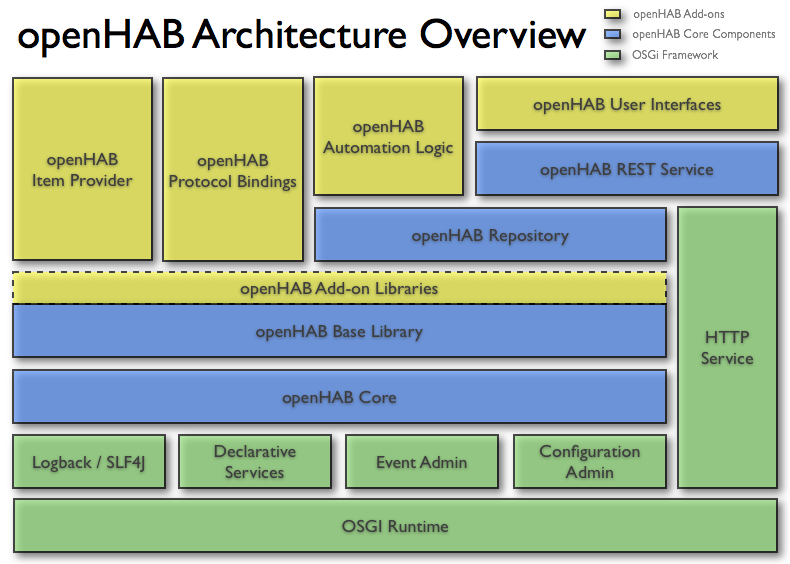
\includegraphics[scale=0.45]{report/img/openHAB_architecture}
	\caption{openHAB Architektur}
	\label{fig:ohArch}
\end{figure}

\subsubsection{Event Bus}
Der Basisservice von openHAB stellt der Event Bus dar. Über diesen Bus werden Events zwischen den verschiedenen OSGI Bundles gesendet. Die Events sind entweder Commands, welche eine Aktion ausführen, oder Status-Updates, welche Zustandsänderungen der Sensoren/Aktoren beinhalten. \\
Durch den Einsatz dieses Event Bus wird die Kopplung reduziert und Add-ons können somit einfach ausgetauscht werden. \\
Intern wurde der Event Bus mit Hilfe des OSGI Event Admin umgesetzt. Durch den Event Admin wird es möglich, dass sich weitere OSGI Bundles (also openHAB Add-ons) im Event Bus einklinken können.

\subsubsection{Bindings}
Bindings sind Verbindungen zwischen openHAB und den externen Systemen und bilden die Grundlage zur Konnektivität. Dadurch muss für jede Technologie ein eigenes Binding geschrieben werden. Für viele Technologien sind Bindings vorhanden, die einzeln heruntergeladen und als «Add-on» installiert werden können. Falls eine Technologie noch nicht unterstützt wird, kann man das Binding dazu selbst programmieren. Die wesentliche Aufgabe besteht darin, sich einerseits mit dem externen Gerät zu verbinden, auf dem Event Bus zu lauschen und die ausgetauschten Daten miteinander kompatibel zu machen. \\
Alle momentan verfügbare Bindings sind unter folgendem Link zu finden: \url{https://github.com/openhab/openhab/wiki/Bindings}

\begin{figure}[H]
	\centering
		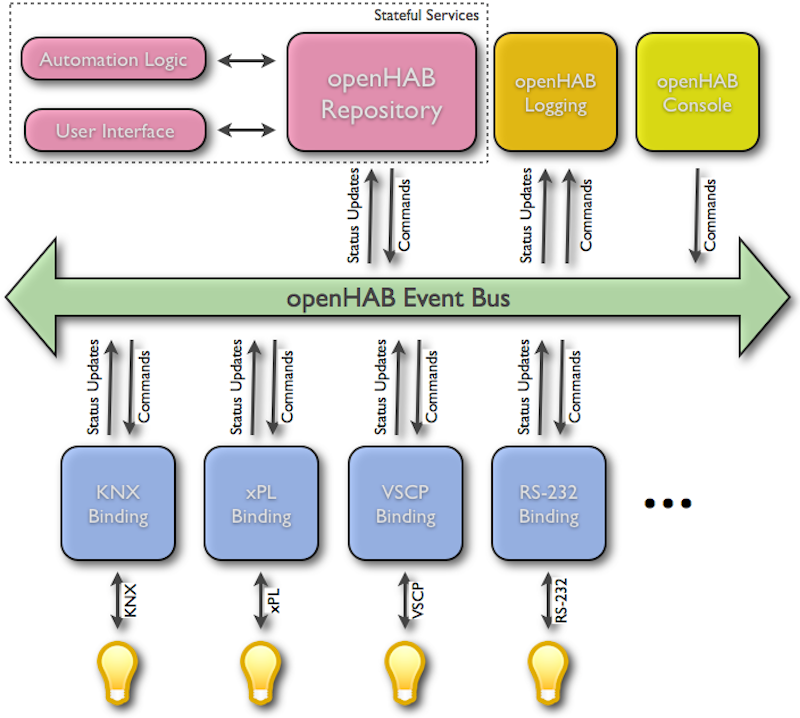
\includegraphics[scale=0.4]{report/img/communicationOH}
	\caption{Event Bus als Schnittstelle für Bindings}
	\label{fig:ohComm}
\end{figure}



\subsubsection{Items}
Wenn so viele unterschiedliche Technologien unterstützt und integriert werden sollen, dann stellt sich die Frage nach dem gemeinsamen Nenner bzw. einer einheitlichen internen Repräsentation. Aus diesem Grund wurden «Items» eingeführt, die zentrale Entität im openHAB Domainmodell. Alle Bindings implementieren ein Mapping zwischen den Daten des Sensors/Aktors und einem zugehörigen Item. Ein Item besteht aus:

\begin{itemize}
	\item Typ
	\item Name
	\item Formatierung
	\item Icon
	\item Gruppe
	\item Bindingparameter
\end{itemize}

Die Eigenschaften Typ und Name sind zwingend, die Anderen sind optional. Der Typ ist auf eine vorgegebene Auswahl beschränkt, der Name dient als Identifier und muss eindeutig sein.\\
\\
Je nach gewähltem Typ können Items die unterschiedlichsten Dinge repräsentieren. Ein sehr häufig verwendeter Typ ist das SwitchItem mit den beiden möglichen Werten ON und OFF. Dieses Item eignet sich aufgrund seines Wertebereichs hervorragend als Boolean. Ein SwitchItem kann stellvertretend für etwas reales, wie eine Lampe, oder für etwas abstraktes wie die Anwesenheit eines Bewohners stehen. Es ist wichtig zu verstehen, dass ein Item rein virtuell ist. Die Brücke zur echten Hardware wird erst über Bindingparameter geschlagen, denn dann verknüpft openHAB das Item mit dem entsprechenden Binding. Da die Bindingparameter eines Items aber optional sind macht openHAB keinen Unterschied zwischen virtuellen und realen Items.


\subsubsection{Item Repository}
Der Zustand eines Items muss die Ausführungsdauer einer openHAB Instanz überleben können, beispielsweise nach einem Neustart. Der Zustand muss ausserdem jederzeit abfragbar sein, egal ob sich der Zustand des Items gerade erst durch ein Event geändert hat oder schon über mehrere Startvorgänge hinweg genau so exisitiert. Diese Verantwortung übernimmt das Item Repository, welches permanent den Event Bus auf Status-Updates abhört und die Änderungen persistiert.

\subsubsection{Rules}
Rules sind die Werkzeuge zur Automatisierung. Dank einer Java-ähnlichen DSL können Aktionen ausgelöst werden, wenn gewisse Bedingungen erfüllt wurden. Das können einerseits Zustandsänderungen von Items, aber auch Systemevents oder Events von selbst angelegten Timern sein. 

\subsubsection{Sitemaps}
Sitemaps sind Konfigurationsfiles zur deklarativen Definition von User Interfaces. Sitemaps werden ebenfalls in einer Xtext basierten DSL geschrieben und haben eine baumartige Struktur. OpenHAB liest das Konfigurationsfile und stellt die Sitemap über eine REST API zur Verfügung. Eine mitgelieferte Webapplikation stellt das User Interface anschliessend im Browser dar. Layouttechnisch orientiert sich die Webapplikation am iOS 6 Design mit Listendarstellung und Drill-Down Prinzip. Die nativen iOS und Android Apps von openHAB verfolgen das selbe Bedienkonzept.\\
Die verschiedenen Elemente, die in Sitemaps verfügbar sind, können Items direkt über deren Name referenzieren. Einige Elemente sind dynamisch und erlauben eine werteabhängige Darstellung.




\pagebreak

\subsection{Konfiguration openHAB}




\subsection{Deploymentübersicht}

\subsubsection{Binding Azure}
\begin{figure}[h!]
	\centering
		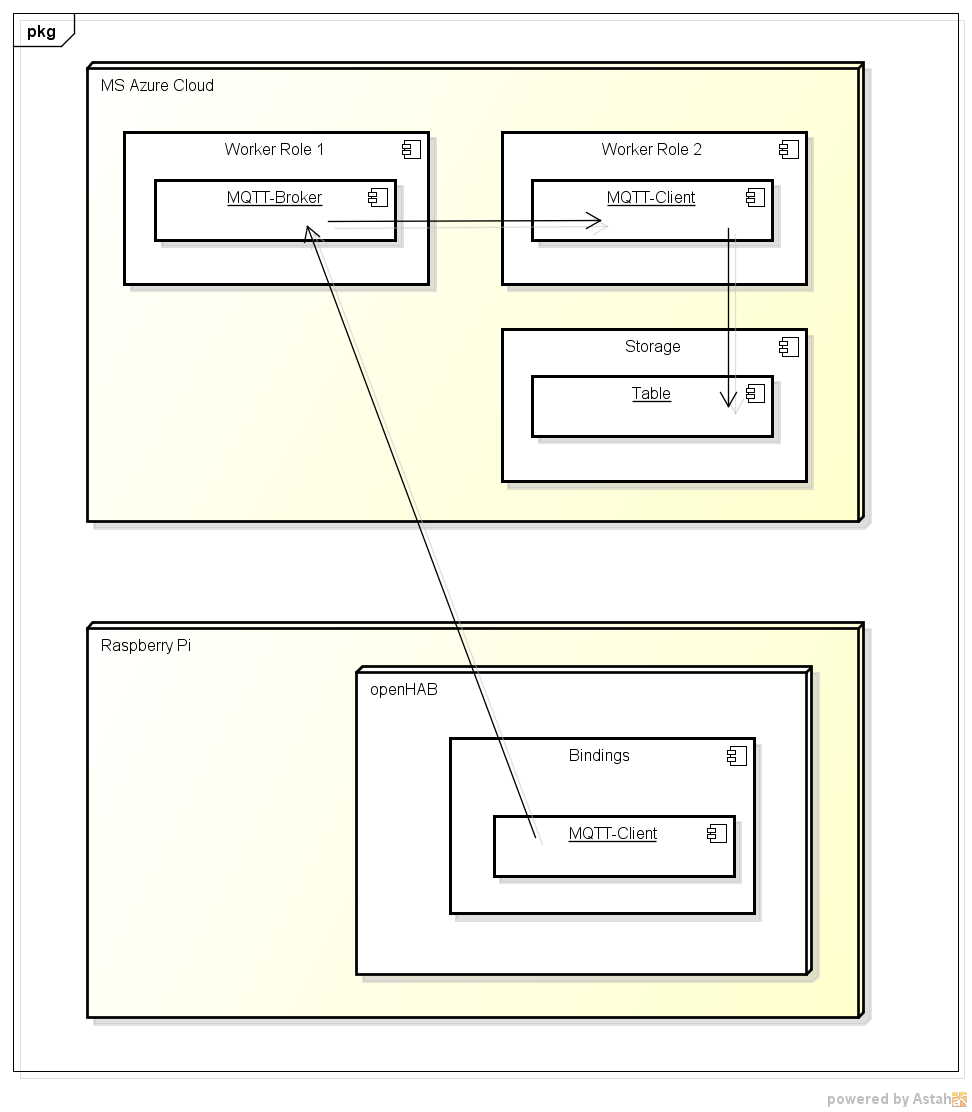
\includegraphics[scale=0.5]{report/img/deployment_binding_azure}
	\caption{Binding Azure Cloud}
	\label{fig:deploymentAzure}
\end{figure}

\subsection{MQTT}
MQTT steht für «Message Queue Telemetry Transport» und ist ein Nachrichten-Protokoll, das speziell für IOT-Anwendungen konzipiert wurde. Es setzt auf dem TCP/IP Stack auf und wird für den Nachrichtenaustausch zwischen verschiedenen, verteilten Maschinen verwendet. \\
Das Protokoll wurde speziell für Systeme designt, die über wenig Speicherplatz und kleiner Netzwerk-Bandbreite verfügen, was bei IOT-Anwendungen meist der Fall ist.

\subsubsection{Funktionsweise}
MQTT folgt dem Prinzip «Publish/Subscribe», sprich Clients können bestimmte Topics abonnieren. Wenn Messages auf dieses Topic gesendet werden, leitet der Broker diese an alle interessierten Clients weiter. \\
In Bezug auf erstellen von Topics agiert der Broker passiv. Das bedeutet, Clients können sich auf beliebigen, selber defnierte, Topics registrieren. Wenn aber niemand auf dieses Topic publiziert, wird der Client nie eine Message erhalten.

\begin{figure}[h!]
	\centering
		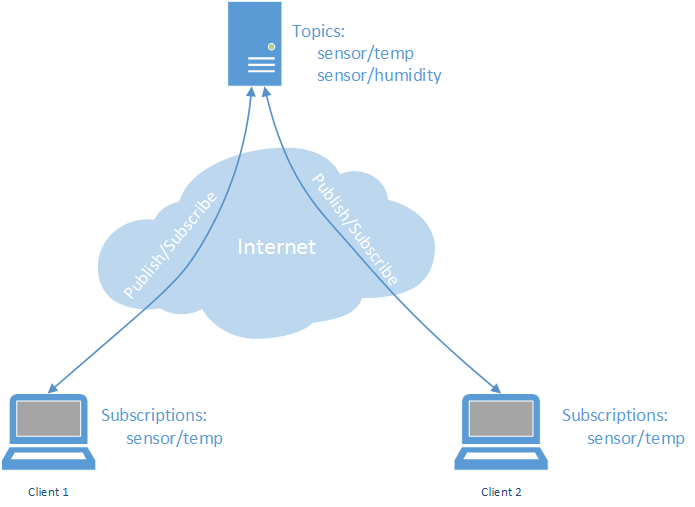
\includegraphics[scale=0.6]{report/img/mqttFunktionsweise}
	\caption{Funktionsweise MQTT}
	\label{fig:deploymentAzure}
\end{figure}

\subsubsection{Broker}

\textbf{Zertifizierungsstelle/Server-Zertifikat} \\
Da die MQTT-Verbindung verschlüsselt werden soll, müssen verschiedene Zertifikate erstellt werden. Das erstellte Server-Zertifikat muss von einer CA (Certification Authority) signiert werden. Da ein gültiges Zertifikat nicht entgeltlich erworben werden möchte, wird eine eigene Zertifizierungsstelle erstellt. OpenSSl bringt da alle nötigen Mittel für die Erzeugung eines CAs mit. Dies bringt den Nachteil mit, dass Computersysteme diesem Zertifikat nicht automatisch trauen, daher muss dann das Zertifkat von Hand dem Certificate Storea als «Trusted Root Certification Authority» hinzugefügt werden. \\

Nachdem die Zertifizierungsstelle erfolgreich generiert wurde, kann das Server Zertifikat erstellt werden. Anschliessend muss dieses Server Zertifikat von der eben erstellten Zertifizierungsstelle signiert werden.

Da sowohl die Zertifizierungsstelle, als auch das Server-Zertifikat auf dem gleichen Computer erstellt werden, muss darauf geachtet werden, dass bei der Erzeugung unterschiedliche Parameter gesetzt werden. Die betroffenen Parameter sind zum Beispiel «Locality Name», «Organizational Name», «Organizational Unit» etc. Falls hier dieselben Werte eingetragen werden, schlägt die Signierung des Serverzertifikates fehl. \\
Weiter muss beachtet werden, dass im Server-Zertifikat der «Common Name» dem FQDN (Fully Qualified Domain Name) des Servers entspricht, auf dem der MQTT-Broker laufen soll. Wird hier beispielsweise nur der Hostname eingetragen, schlägt die Überprüfung des Zertifikates fehl, da sich der CN vom FQDN des Servers unterscheidet.

\textbf{Installation und Konfiguration des Brokers} \\
Wie bereits im Lösugnskonzept erarbeitet, wird als MQTT-Broker «Mosquitto» eingesetzt. Der Broker kann als Binary installiert und über die Commandline gestartet werden.
Nach der Standard-Installation muss der Broker Konfiguriert werden. Dazu wird das File «mosquitto.conf» bearbeitet.
\\Folgende Parameter müssen editiert werden:

\begin{tabularx}{\textwidth}{lX}
		\textbf{Parameter} & \textbf{Erklärung}
		\\ \hline
			bind\_address \tbd &
			IP-Adresse, an den der Default-Listener gebunden wird.
		\\ \hline
			port 8883 &
			Port, auf den der Default-Listener hören soll. Wenn er nicht speziell definiert wird, hört der Listener per Default auf den Port 1883. Da aber mit TLS verschlüsselt wird, muss dieser von Hand auf den dafür vorgesehenen Port 8883 gesetzt werden.
		\\ \hline
			cafile \tbd &
			Hier wird der Pfad eingetragen für das zuvor erstellte CA-Zertifikat.
		\\ \hline
			certfile \tbd &
			Hier wird der Pfad eingetragen für das PEM-Encodete Server Zertifikat.
		\\ \hline
			keyfile \tbd &
			Hier wird der Pfad eingetragen für das PEM-Encodete Keyfile.
		\\ \hline
			tls\_version tlsv1 &
			Diese Option definiert die zu verwendende TLS-Version. Für Openssl (Version 1.0.2) wird tlsv1 verwendet.
		\\ \hline
\end{tabularx}

\subsubsection{Client (Azure Worker Role)}
Wie die Abbildung \ref{fig:systemView} (Systemübersicht) zeigt, befindet sich nebst dem Broker auch ein Client, in form einer Worker Role, in der Cloud. Die Worker Role abonniert alle Topics und persistiert die Messages im Table bzw. Blob-Storage.

In der \lstinline!OnStart()!-Methode der Worke Role werden zu erst die Referenzen zum Table- und Blob-Storage erzeugt. \\
Danach wird die Verbindung zum MQTT-Broker hergestellt, die Topics definiert, die er abonnieren möchte und der QoS-Level gesetzt. \\
Damit der Client benachrichtigt wird, wenn eine Message eintrifft, wird der Eventhandler \lstinline!client_MqttMsgPublishReceived()! definiert. Die Methode muss die gleichen Parameter entgegennehmen, wie die Delegate-Methode. Das ist einerseits der Sender (Object) und die Event-Argumente. Damit der Eventhandler beim Eintreffen einer Message aufgerufen wird, muss dieser auf dem Event registriert werden: \\ \lstinline!client.MqttMsgPublishReceived += client_MqttMsgPublishReceived;! 

\begin{lstlisting}[style=csharp]
public override bool OnStart()
{
  setupStorageConnections();
  MqttClient client = new MqttClient(
            				"mqttbrokerba.cloudapp.net",
               				8883, true, null
               			  );
  client.MqttMsgPublishReceived += client_MqttMsgPublishReceived;
  client.Connect(Guid.NewGuid().ToString(),
  				 "mosquitto",
  				 "baIOT_mq++"
  				 );
  string[] topics = { "openhab/+" };
  byte[] qos = { MqttMsgBase.QOS_LEVEL_EXACTLY_ONCE };
  client.Subscribe(topics, qos);

  return result;
}
\end{lstlisting}

Im Eventhandler wird dann schlussendlich die Logik zur Persistierung eingefügt. Wenn eine Message über das Topic «openhab/blob» empfangen wird, handelt es sich um eine Fotografie der Webcam. Dieses JPG-File wird als Byte-Array übermittelt und wird so auch im Blob-Storage abgelegt. \\
Bei allen anderen Messages muss es sich um Text handeln, daher werden sie im Table-Storage abgelegt.

\begin{lstlisting}[style=csharp]
void client_MqttMsgPublishReceived(object sender,
								   		MqttMsgPublishEventArgs e)
{
	if (e.Topic.Equals("openhab/blob"))
	{
		CloudBlockBlob blockBlob = container.
							GetBlockBlobReference(Guid.NewGuid()
								   							.ToString());
		blockBlob.UploadFromByteArray(e.Message,
									  0, e.Message.Length);
    }
	else
	{
    	var message = System.Text.Encoding.
    							  Default.GetString(e.Message);
		Entity entity = new Entity(message);
		TableOperation insertOperation = TableOperation.
											Insert(entity);
		table.Execute(insertOperation);
	}
}
\end{lstlisting}










